\chapter{Pre-Exploitation}
\markboth{Pre-Exploitation}{}

\section{Target Scoping}
In questa fase bisogna stipulare un accordo tra le parti (responsabile dell'asset e pentester) in modo da definire vincoli, limiti, responsabilità legali in caso di eventuali problemi, accordo di non divulgazione, ecc. Tuttavia, si possono fare le seguenti osservazioni:

\begin{itemize}
    \item L'asset da analizzare è pubblicamente disponibile e realizzato appositamente per essere analizzato, ossia vulnerabile by-design;
    \item Tutta l'analisi avviene in un ambiente virtualizzato all'interno della macchina in possesso al Penetration Tester;
    \item Lo scopo dell'analisi è puramente didattico, in quanto realizzato in un contesto universitario e, più precisamente, come progetto del corso "Penetration Testing and Ethical Hacking";
    \item Tutti gli strumenti utilizzati e le fonti consultate sono pubblicamente disponibili e accessibili o, in generale, sono accessibili tramite piani gratuiti e quindi senza costi da sostenere.
\end{itemize}

In conclusione, come si può notare dalle precedenti osservazioni, questa fase può essere tranquillamente saltata visto che non ci sono parti con cui prendere accordi e non possono esserci problematiche di tipo legale dal momento che l'ambiente è totalmente simulato.

\section{Information Gathering}
Durante questa fase, l'obiettivo è quello di trovare più informazioni possibili riguardo l'asset scelto e, essendo che l'asset è una macchina virtuale che viene eseguita in un \emph{ambiente virtualizzato} e in una \emph{rete con NAT virtuale} (come illustrato nell'introduzione), si eviteranno fonti e tool che raccolgono informazioni riguardo persone afferenti all'organizzazione dell'asset, indirizzi e-mail, analisi di record DNS, informazioni di routing e così via. A questo punto, l'unica tecnica che ha senso utilizzare (e che è stata effettivamente utilizzata) è \textbf{OSINT} (\emph{Open Source INTelligence}), con cui si cercherà di individuare nomi utente, password, indirizzo IP, ecc. Tutto questo, ovviamente, evitando di consultare fonti dove sono presenti Walktrough e guide per evitare di vanificare il contributo didattico del processo.

Come primo passo, è stata consultata la pagina di Vulnhub sulla quale sono riportate varie informazioni riguardo la macchina virtuale scelta "\textbf{De-ICE S1.140}" e,
all'interno della pagina, sono state trovate le seguenti informazioni:
\begin{itemize}
    \item Informazioni riguardo il \textbf{rilascio}, ovvero autore, data, sorgente e valore hash della macchina. Queste informazioni, tuttavia, non sembrano essere utili per il processo;
    \item Una \textbf{descrizione} molto ad alto livello della macchina. Anche qui non viene rilasciata alcuna informazione utile come servizi esposti dalla macchina o credenziali di accesso alla macchina (anche non privilegiate). Infatti, attualmente, se si avvia la macchina non si può fare nulla tramite \emph{interazione diretta} in quanto \textbf{non è stata rilasciata nessuna credenziale di accesso};
    \item Informazioni riguardo la configurazione dell'\textbf{indirizzo di rete}. Questa informazione è molto utile perché ci rivela che la macchina \textbf{non è configurata per lavorare con un indirizzo IP specifico} ma lo ottiene in maniera automatica grazie al servizio \textbf{DHCP}. Questo ci fa subito capire che all'interno della rete con NAT non avremo problemi di indirizzamento ma, sfortunatamente, questo significa che non si può conoscere apriori l'indirizzo della macchina (l'unica certezza è che sarà all'interno della rete \emph{10.0.2.0/24}) ma dovremo ricavarcelo in maniera indiretta visto che \emph{VirtualBox} non fornisce un metodo diretto di ottenimento degli indirizzi IP e \textbf{non è possibile l'accesso alla macchina};
    \item Informazioni riguardo il \textbf{sistema operativo}. Altra informazione molto utile in quanto adesso si è a conoscenza che l'asset è un sistema Linux e questo ci permetterà di risparmiare tempo in fasi avanzate perché si può restringere il campo delle scansioni solo a sistemi Linux, escludendo tutti gli altri. Tuttavia, non si conosce ancora la versione precisa del kernel e quindi si deve ricavare successivamente;
\end{itemize}

Andando più a fondo nella pagina si può ricavare l'indirizzo del \textbf{sito web del creatore} dell'asset e il \textbf{link di download della macchina} ma, sfortunatamente, entrambi i link \textbf{non sono più attivi}. Consultando il motore di ricerca Google, semplicemente ricercando il nome dell'organizzazione trovato sulla pagina, è possibile risalire al rispettivo account Twitter e si nota che quest'ultimo non è attivo all'incirca dal 2020. Per questa ragione, è sembrato opportuno accedere al servizio \emph{WaybackMachine} offerto da \textbf{Archive.org} per visitare versioni precedenti del sito dell'organizzazione nella speranza di trovare altre informazioni utili. Fortunatamente, grazie a questo servizio è stato possibile accedere ad uno \emph{snapshot} risalente al 2021 dal quale è stato anche possibile effettuare il download della macchina. Ad ogni modo, anche accedendo al sito e, in particolare, alla pagina di download, non sono state trovate informazioni rilevanti come credenziali, porte aperte, schemi di naming, ecc.

\section{Target Discovery}
In questa fase si avvieranno entrambe le macchine e si procederà con la scansione della rete \emph{Corso}, con lo scopo di trovare tutte le macchine attive all'interno della stessa. Ovviamente ci si aspetta di trovare solo la macchina \textbf{De-ICE S1.140} e la macchina \textbf{Kali} per come è stato impostato l'ambiente.

\subsection{Esecuzione di \texttt{ifconfig}}
Prima di cominciare con la scansione effettiva della rete, bisogna capire qual è l'indirizzo della macchina \textbf{Kali} in modo da escludere il suo IP da successive scansioni più approfondite. Per ottenere questa informazione ci basta semplicemente lanciare il comando \texttt{ifconfig} e,una volta lanciato questo comando, si ottiene il seguente output:
\begin{figure}[h]
    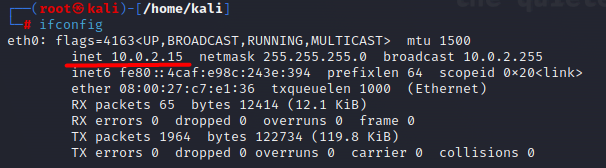
\includegraphics[width=0.8\textwidth]{capitoli/figure/ifconfig-kali.png}
    \centering
    \caption{Esecuzione di \texttt{ifconfig} su Kali}
    \label{fig:ifconfig}
\end{figure}

Come si può notare dall'output, l'indirizzo di Kali è \emph{10.0.2.15} e, adesso che si ha quest'informazione, si può cominciare con la scansione della rete.
\subsection{Scansione con \texttt{nmap}}
Il primo strumento utilizzato per la scansione è \texttt{nmap}, un potentissimo strumento di scansione che tornerà molto utile anche nelle successive fasi. In particolare, tra le varie tipologie che offre \texttt{nmap}, permette anche di eseguire una scansione di tipo \textbf{ICMP} (detta \emph{ping scan} \cite{nmap-doc}) su una determinata sottorete presa in input. Con questa scansione, \texttt{nmap} invierà a tutti gli indirizzi specificati dei pacchetti \emph{ICMP Echo Request} e, se prima dello scadere di un timeout prefissato, riceve da un host un pacchetto \emph{ICMP Echo Reply}, \texttt{nmap} capirà che l’host è attivo e risponde altrimenti marcherà quell’indirizzo come non attivo. Per eseguire una \emph{ping scan} sulla rete \emph{Corso} basta lanciare il seguente comando:

\begin{lstlisting}[language=bash]
    nmap -sP 10.0.2.0/24
\end{lstlisting}

Una volta lanciato questo comando, è possibile osservare il seguente output:
\begin{figure}[h]
    \centering
    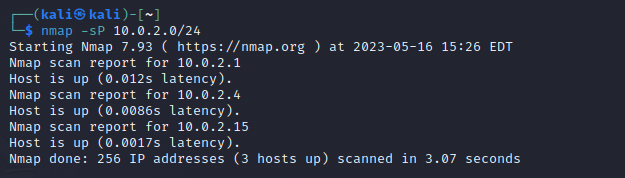
\includegraphics[width=0.8\textwidth]{capitoli/figure/discovery-nmap.png}
    \caption{Risultato della \emph{ping scan} con \texttt{nmap}}
    \label{fig:nmap-ping-scan}
\end{figure}

Il primo dato che dovrebbe risaltare è che il numero degli host attivi sulla rete è 3, e non 2 come in realtà ci si aspettava dalla configurazione realizzata. Tuttavia, come specificato a lezione e approfondito anche nella documentazione di \emph{VirtualBox}, all'interno della rete saranno presenti uno o più host "\emph{fittizi}" che sono necessari allo stesso \emph{VirtualBox} per realizzare la stessa \emph{rete con NAT} \cite{virtualbox-nat}. Questi host di solito hanno sempre i primi indirizzi assegnabili, quindi è lecito pensare che l'host con indirizzo \emph{10.0.2.1} sia proprio l'host interno di \emph{VirtualBox} e che l'host con indirizzo \emph{10.0.2.4} sia il nostro asset. Per quanto riguarda \emph{10.0.2.15}, in realtà già si conosce dal comando lanciato prima e si sa per certo che è proprio l'indirizzo della macchina \textbf{Kali}.

\subsection{Scansione con \texttt{arp-scan}}
Grazie ad \texttt{nmap} si conoscono gli indirizzi IP degli host attivi all'interno della rete, però in seguito potremmo essere interessati anche agli indirizzi \emph{MAC} corrispondenti. Questo perchè l'infrastruttura di rete è composta da un solo \emph{router virtuale} al quale si collegano tutti gli host (come indicato anche nella Figura \ref{fig:infrastruttura-kali}) e, per questa ragione, è possibile utilizzare anche il protocollo \textbf{ARP} essendo una rete locale. A tal proposito, è stato utilizzato il tool \texttt{arp-scan} che, sfruttando proprio il protocollo \textbf{ARP}, è in grado di ottenere gli indirizzi \emph{MAC} degli host connessi \cite{arp-scan-doc}. Per eseguire lo strumento sulla rete, è necessario eseguire il seguente comando:

\begin{lstlisting}[language=bash]
    arp-scan 10.0.2.0/24
\end{lstlisting}

Una volta eseguito questo comando, l'output che viene fornito è il seguente:

\begin{figure}[h]
    \centering
    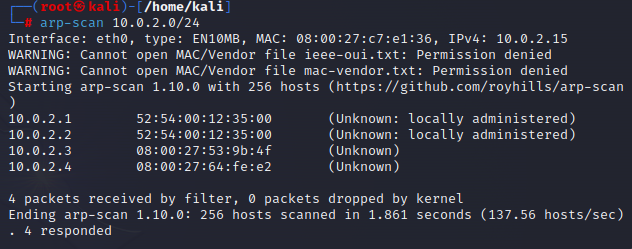
\includegraphics[width=0.8\textwidth]{capitoli/figure/arp-scan.png}
    \caption{Risultato della scansione con \texttt{arp-scan}}
    \label{fig:arp-scan-risultato}
\end{figure}

Anche qui è possibile notare subito un'altra anomalia. Con \texttt{nmap} sono stati rilevati 3 host invece di 2, mentre adesso con \texttt{arp-scan} ne sono stati rilevati persino 5 (includendo anche la macchina \textbf{Kali} nel conteggio). Osservando con attenzione il risultato, si può notare che gli indirizzi \emph{10.0.2.1} e \emph{10.0.2.2} facciano riferimento allo stesso indirizzo MAC (quindi una singola interfaccia con due indirizzi distinti), avvalendo la supposizione precedente che facciano riferimento ad un singolo host interno di \emph{VirtualBox}. A questo punto, se si continua a seguire la supposizione che \emph{10.0.2.4} sia l'asset, allora si può dire che \emph{10.0.2.3} è un altro host interno di \emph{VirtualBox}. Quindi in realtà gli host attivi non sono 5 come poteva sembrare inzialmente ma sono soltanto 4, e 2 di questi sono host interni di \emph{VirtualBox}.
\subsection{Ulteriore scansione con \texttt{nping}}
A questo punto può sorgere un dubbio, sono stati effettivamente scovati tutti gli host sia "\emph{reali}" che "\emph{fittizi}"? Per acquisire più sicurezza nell'identificarli tutti, evitando così ulteriori sorprese, vale la pena di effettuare un'ulteriore scansione della rete. Per realizzare questa ulteriore scansione è stato utilizzato il tool \texttt{nping}, il quale genererà pacchetti \emph{ICMP} in maniera molto simile al comando \texttt{ping} su tutti gli host forniti in input (quindi ancora una \emph{ping scan} \cite{nping-man}). Per effettuare una scansione con questo tool basta lanciare il seguente comando:

\begin{lstlisting}[language=bash]
    nping -c 1 10.0.2.0/24
\end{lstlisting}

Una volta lanciato il comando si ottiene il seguente output:
\begin{figure}[h]
    \begin{subfigure}{0.5\textwidth}
        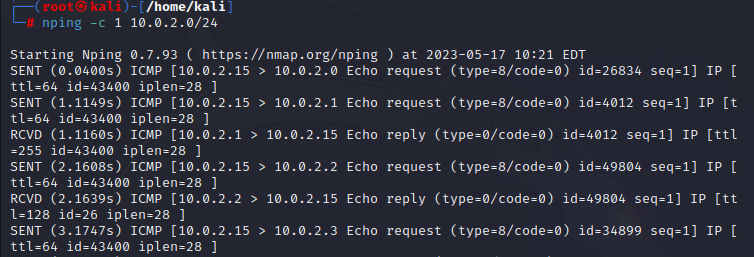
\includegraphics[width=1\textwidth]{capitoli/figure/nping-esecuzione-parziale.png}
        \caption{Esecuzione parziale di \texttt{nping}}
        \label{fig:nping-esecuzione-parziale}
    \end{subfigure}
    \begin{subfigure}{0.5\textwidth}
        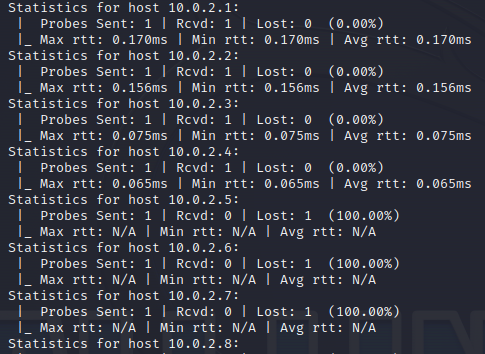
\includegraphics[width=1\textwidth]{capitoli/figure/nping-risultato-parziale.png}
        \caption{Risultato parziale di \texttt{nping}}
        \label{fig:nping-risultato-parziale}
    \end{subfigure}
    \begin{subfigure}{0.9\textwidth}
        \centering
        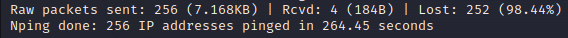
\includegraphics[width=1\textwidth]{capitoli/figure/nping-statistiche.png}
        \caption{Statistiche di \texttt{nping}}
        \label{fig:nping-statistiche}
    \end{subfigure}
    \caption{Output di \texttt{nping}}
\end{figure}

Osservando l'output fornito dal tool \texttt{nping}, sembra che sia conforme con le informazioni ottenute mettendo insieme le precedenti due scansioni. Infatti, si può notare dalla Figura \ref{fig:nping-risultato-parziale} che a rispondere al ping sono gli indirizzi \emph{10.0.2.1-4} confermando quindi che sulla rete sono attivi solo 4 host (contando anche la macchina \textbf{Kali}).

\subsection{OS Fingerprinting con \texttt{nmap}}
Con quest'ultima scansione è terminata l'identificazione degli host attivi sulla rete e, per questo motivo, si può passare al passo successivo. Durante la fase di \emph{Information Gathering} è stato possibile stabilire che l'asset è una macchina Linux, ma senza conoscere la versione effettiva del kernel. A tal proposito si può utilizzare ancora una volta il tool \texttt{nmap} che, tramite una tipologia di scansione particolare, è in grado di fare \textbf{OS Fingerprinting} di una determinata macchina presa in input \cite{nmap-doc}. Per fare ciò, basta eseguire il seguente comando:

\begin{lstlisting}[language=bash]
    nmap -O 10.0.2.4
\end{lstlisting}

Una volta eseguito, l'output ottenuto è il seguente:
\begin{figure}[h]
    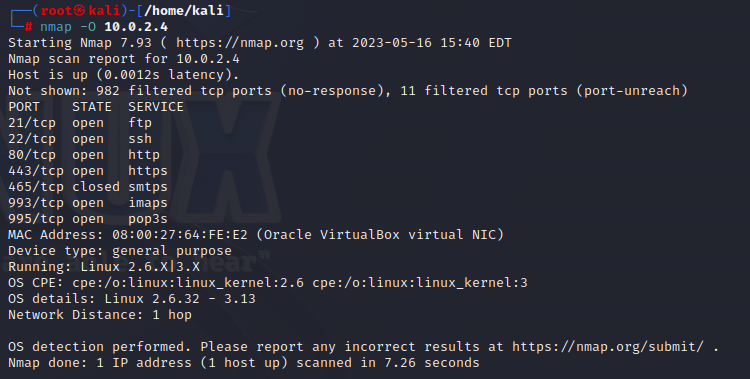
\includegraphics[width=1\textwidth]{capitoli/figure/nmap-os-fingerprint.png}
    \centering
    \caption{Risultato dell'OS Fingerprinting con \texttt{nmap}}
    \label{fig:nmap-os-fingerprint}
\end{figure}

Si può notare che la versione del kernel identificata da \texttt{nmap} risulta essere la \emph{2.6.x/3.x}, in particolare potrebbe trattarsi della versione \emph{2.6.32} o \emph{3.13}. Oltre all'\textbf{OS fingerprint}, è possibile notare che \texttt{nmap} ha eseguito anche una scansione delle porte attive sull'host target. Ovviamente si è limitato solo alle mille più frequenti \cite{nmap-doc} (e per questo sarà necessaria una scansione più approfondita nella fase successiva), tuttavia, si può visualizzare che ha delle porte aperte le quali possono essere molto interessanti anche in questo momento. In particolare, le suddette porte sono quelle relative a \textbf{ftp}, \textbf{ssh} e \textbf{http} e, sono particolarmente interessanti poichè si può pensare ad un approfondimento.

\subsection{OS Fingerprint passivo con \texttt{p0f}}
Come accennato in precedenza, grazie a quelle porte aperte si può pensare di fare un'ulteriore scansione ma, questa volta, di tipo passivo. Si può pensare di utilizzare il tool \texttt{p0f}, che si occupa di analizzare il traffico "legittimo" generato da e verso i vari host facendo \emph{pattern matching} con delle \textbf{firme} \cite{p0f-man}. Quindi, tutto quello che bisogna fare è eseguire il comando \texttt{p0f} e lasciarlo in backround nel mentre che si genera del traffico "legittimo" verso l'asset.

Un primo tentativo che si può fare è quello di generare del traffico \emph{ftp} verso la macchina e, successivamente, controllare se \texttt{p0f} è riuscito ad estrapolare informazioni utili:

\begin{figure}[h]
    \begin{subfigure}{0.5\textwidth}
        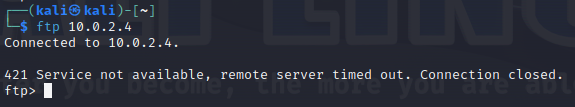
\includegraphics[width=1\textwidth]{capitoli/figure/kali-ftp.png}
        \caption{Generazione di traffico \emph{ftp} legittimo}
        \label{fig:kali-ftp}
    \end{subfigure}
    \begin{subfigure}{0.5\textwidth}
        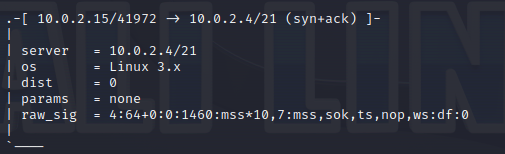
\includegraphics[width=1\textwidth]{capitoli/figure/p0f-ftp.png}
        \caption{Risultato analisi di \texttt{p0f} su traffico \emph{ftp}}
        \label{fig:p0f-ftp}
    \end{subfigure}
\end{figure}

Come si può notare dalla Figura \ref{fig:p0f-ftp}, \texttt{p0f} analizzando il traffico \emph{ftp} è stato in grado di stabilire che il sistema operativo dell'asset ha una versione del kernel \emph{3.x}. Essendo che le tecniche passive non hanno la stessa accuratezza dei metodi attivi (non inviano pacchetti \emph{ad-hoc}), invece di concludere l'analisi con questa informazione è meglio approfondire ulteriormente. A tal proposito, questa volta si è generato del traffico \emph{http} sfruttando il browser \textbf{Mozilla Firefox} installato su \textbf{Kali}. Senza interrompere l'esecuzione di \texttt{p0f}, una volta generato il suddetto traffico è stato ottenuto il seguente output:

\begin{figure}[h]
    \centering
    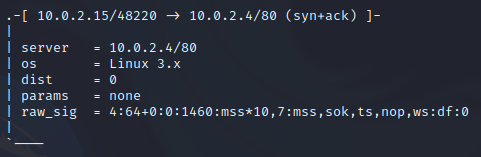
\includegraphics[width=0.7\textwidth]{capitoli/figure/p0f-http.png}
    \caption{Risultato analisi di \texttt{p0f} su traffico \emph{http}}
    \label{fig:p0f-http}
\end{figure}

Consultando anche questo risultato, si può notare che anche qui \texttt{p0f} ha identificato il kernel \emph{3.x}, rendendo più plausibile questa come versione effettiva.

Inoltre, unendo quest'informazione con la scansione attiva realizzata da \texttt{nmap}, è lecito dedurre che molto probabilmente la versione del kernel utilizzata dall'asset sia proprio la versione \emph{3.13}.

\section{Target Enumeration}
Adesso che si è a conoscenza della versione del kernel e dell'indirizzo dell'asset, si può procedere con una scansione più approfondita per conoscere i servizi offerti e le porte aperte. Si eseguirà prima una scansione utilizzando il protocollo \emph{TCP} e successivamente si realizzerà una scansione utilizzando il protocollo \emph{UDP}. 
\subsection{\emph{TCP} Port Scanning}
\subsubsection{Esecuzione di \texttt{nmap -sS}}
Per scovare le porte che sono aperte sull'asset viene effettuata una \emph{SYN Scan} sfruttando \texttt{nmap}, ovvero la macchina \textbf{Kali} invierà un pacchetto \emph{SYN} su ogni porta specificata e, in base alla risposta ricevuta, \texttt{nmap} interpreterà la porta come \emph{aperta}, \emph{chiusa} o \emph{filtrata}. Per realizzare questo tipo di scansione basta lanciare il seguente comando:

\begin{lstlisting}[language=bash]
    nmap -sS -p- 10.0.2.0/24
\end{lstlisting}
dove con l'argomento \texttt{-p-} si specificano tutte le porte \cite{nmap-doc}.

In seguito all'esecuzione del comando, l'output è il seguente:

\begin{figure}[h]
    \centering
    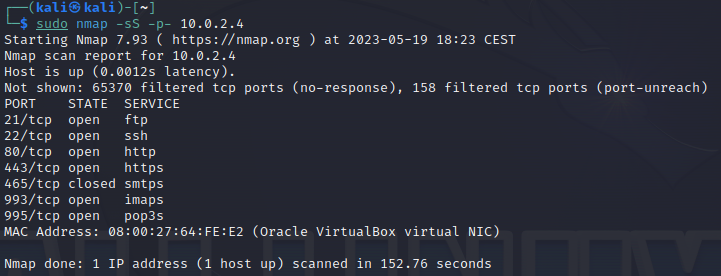
\includegraphics[width=1\textwidth]{capitoli/figure/nmap-syn-scan.png}
    \caption{Risultato della \emph{SYN Scan} con \texttt{nmap}}
    \label{fig:nmap-syn}
\end{figure}

Analizzando il risultato ottenuto, il primo dato che risalta è che le porte rilevate come aperte sono uguali a quelle individuate già in precedenza (Figura \ref{fig:nmap-os-fingerprint}), mentre il secondo è che tutte le porte restanti sono \textbf{filtrate} e non \textbf{chiuse}. Questo risultato ci porta a supporre la presenza di un \textbf{Firewall/IDS} sulla macchina e questo richiede un ulteriore approfondimento.

\subsubsection{Esecuzione di \texttt{nmap -sF}}
Un approfondimento che si può tentare è quello di eseguire una tipologia di scansione che sia diversa dalla \emph{SYN Scan}, anche per stabilire se i meccanismi di filtraggio agiscono solo su pacchetti di tipo \textbf{SYN}. Una tipologia di scansione che vale la pena di tentare è la \emph{FIN Scan}, ovvero una scansione dove invece di inviare pacchetti \textbf{SYN} vengono inviati pacchetti \textbf{FIN}. Tuttavia, questa tipologia di scansione è meno precisa perchè se non riceve risposta non riesce a distinguere se la porta interrogata è aperta o filtrata (per via dell'attesa, ovviamente, è molto più lenta rispetto alla \emph{SYN Scan}), ma se riceve una risposta di tipo \emph{RST} o \emph{ICMP Port Unreachable} riesce correttamente a dire che la porta è chiusa \cite{nmap-doc}. Per eseguire questo tipo di scansione basta eseguire il seguente comando:

\begin{lstlisting}[language=bash]
    nmap -sF -T5 -p- 10.0.2.4
\end{lstlisting}

Una volta eseguito, il risultato ottenuto è il seguente:

\begin{figure}[h]
    \centering
    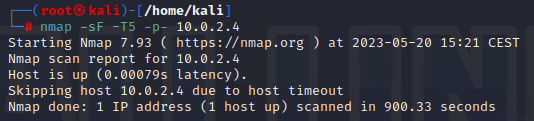
\includegraphics[width=1\textwidth]{capitoli/figure/nmap-fin-scan.png}
    \caption{Risultato della \emph{FIN Scan} con \texttt{nmap}}
    \label{fig:nmap-fin}
\end{figure}

Come si evince immediatamente, dopo 15 minuti di attesa la scansione è terminata per via del \emph{timeout} di default impostato da \texttt{nmap} non portando alcun risutato significativo.

\subsubsection{Esecuzione di \texttt{nmap -sA}}
Un ulteriore strategia da seguire è quella di effettuare un tipo di scansione diversa che sia più diretta all'individuazione di meccanismi di filtraggio. Una scansione adatta allo scopo è la \emph{ACK Scan}, che è più complessa da bloccare e consiste nell'inviare pacchetti solo con il flag \emph{ACK} aspettandosi in ritorno un pacchetto \emph{RST} nel caso in cui la porta è aperta o chiusa (se non riceve risposta o riceve un pacchettp \emph{ICMP} allora la porta è filtrata \cite{nmap-doc}). Per iniziare questo tipo di scansione basta eseguire il seguente comando:

\begin{lstlisting}[language=bash]
    nmap -sA -T5 -p- 10.0.2.4
\end{lstlisting}
dove con l'opzione \texttt{-T5} si specifica un opzione di temporizzazione che indica ad \texttt{nmap} di andare alla massima velocità possibile. Non c'è il rischio di causare problemi di rete all'asset adottando questo comportamento poichè esso si trova in un ambiente simulato.

In seguito all'esecuzione del comando, l'output è il seguente:
\begin{figure}[h]
    \centering
    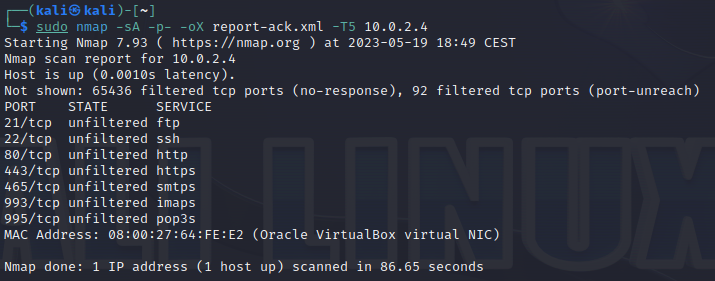
\includegraphics[width=1\textwidth]{capitoli/figure/nmap-ack-scan.png}
    \caption{Risultato della \emph{ACK Scan} con \texttt{nmap}}
    \label{fig:nmap-ack}
\end{figure}

Come è evidente dal risultato ottenuto, non si può che confermare la presenza di un meccanismo di filtraggio sull'asset.

\subsubsection{Esecuzione di \texttt{nmap -sV}}
A questo punto, ponendo l'attenzione solo sulle porte aperte, il prossimo passo da effettuare è quello di stabilire quali sono i servizi associati alle varie porte e quali sono le versioni di questi. Per questa tipologia di compito, è necessaria una scansione di tipo \emph{Version Detection} che ha lo scopo di inviare pacchetti specifici e confrontare le risposte ottenute con delle \textbf{firme} specifiche \cite{nmap-doc}. Per eseguire questo tipo di scansione e ottenere anche un report dettagliato basta eseguire il seguente comando:

\begin{lstlisting}[language=bash]
    nmap -sV -p- -oX report.xml -T5 10.0.2.4
\end{lstlisting}

Una volta eseguito il comando, l'output sarà il seguente:

\begin{figure}[h]
    \centering
    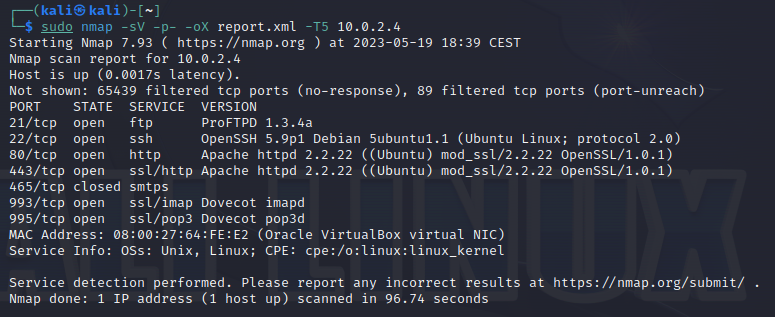
\includegraphics[width=1\textwidth]{capitoli/figure/nmap-version-scan.png}
    \caption{Risultato della \emph{Version Detection} con \texttt{nmap}}
    \label{fig:nmap-version}
\end{figure}

Il report dettagliato della scansione è stato esportato in formato \emph{XML} e successivamente convertito in formato \emph{HTML} per una consultazione più agevole. Ad ogni modo, dal report si evince che alle porte aperte corrispondono i servizi che convenzionalmente sono esposti su di esse ed \texttt{nmap} è stato in grado di risalire anche alle versioni di quasi tutti i servizi esposti.

\subsubsection{Esecuzione di \texttt{nmap -A}}
Un raffinamento della \emph{Version Detection} precedente si può ottenere eseguendo una tipologia particolare di scansione offerta da \texttt{nmap}. Questa scansione è chiamata \emph{Aggressive Scan} ed è una scansione che esegue contemporaneamente le seguenti scansioni:
\begin{itemize}
    \item \textbf{Version Detection}
    \item \textbf{OS Fingerprinting}
    \item \textbf{Traceroute}
    \item \textbf{Script Scan}
\end{itemize}
L'ultima in particolare è una scansione che esegue gli script appartenenti alla categoria \emph{default} di \texttt{nmap}. Questi possono tornare molto utili poichè in grado recuperare molte più informazioni di quante potrebbe ricavare la \emph{Version Detection} da sola \cite{nmap-doc}. Per eseguire questa tipologia di scansione e ottenere un report dettagliato basta eseguire il seguente comando:

\begin{lstlisting}[language=bash]
    nmap -A -T5 -p- -oX report-aggressive.xml 10.0.2.4
\end{lstlisting}

Una volta eseguito, il risultato sarà il seguente:

\begin{figure}[h]
    \centering
    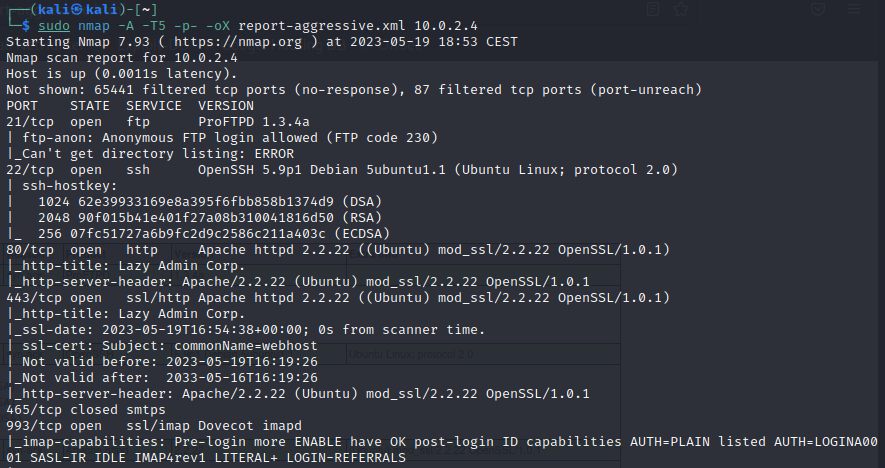
\includegraphics[width=1\textwidth]{capitoli/figure/nmap-aggressive-scan.png}
    \caption{Risultato della \emph{Aggressive Scan} con \texttt{nmap}}
    \label{fig:nmap-aggressive}
\end{figure}

Rispetto alla semplice \emph{Version Detection}, grazie agli \textbf{script} eseguiti durante la scansione sono state recuperate altre informazioni che potrebbero tornare utili come chiavi \emph{SSH}, possibilità di accesso anonimo su \emph{FTP}, ecc. Il report dettagliato è stato esportato e converito in \emph{HTML} per una consultazione più agevole.

\subsection{\emph{UDP} Port Scanning}

\subsubsection{Esecuzione di \texttt{unicornscan}}
Terminata la scansione delle porte \emph{TCP}, il prossimo passo da eseguire è la scansione delle porte \emph{UDP}. Per realizzare questo passo è stato utilizzato \texttt{unicornscan}, il quale supporta le scansioni di tipo \emph{UDP} e permette di impostare il numero di \textbf{pacchetti al secondo} da inviare per realizzare la scansione \cite{unicornscan-doc}. Per effettuare una scansione sull'asset basta eseguire il seguente comando:

\begin{lstlisting}[language=bash]
    unicornscan -m U -Iv 10.0.2.4:1-65535 -r 1000
\end{lstlisting}
dove con \texttt{-m U} si indica che la scansione da eseguire userà il protocollo \emph{UDP}, con \texttt{-Iv} si forza la visualizzazione dei risultati appena questi sono disponibili e che attiviamo la modalità \emph{verbose} (vengono stampati anche output non necessari ai fini del risultato finale) e, infine con \texttt{-r} si indica il numero di pacchetti al secondo da inviare \cite{unicornscan-man}.

Una volta eseguito il comando, l'output sarà il seguente:

\begin{figure}[h]
    \centering
    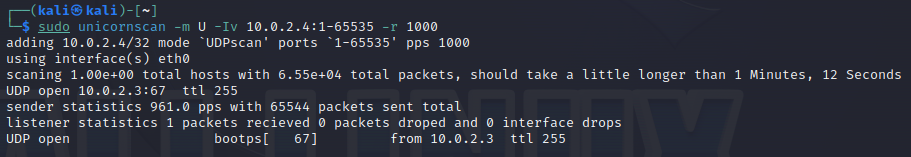
\includegraphics[width=0.8\textwidth]{capitoli/figure/unicornscan-all-ports.png}
    \caption{Risultato scansione \emph{UDP} con \texttt{unicornscan}}
    \label{fig:unicornscan-scan}
\end{figure}

Come è possibile notare dal risultato ottenuto viene riscontrata una porta \emph{UDP} aperta ma, se osserviamo attentamente, questa si trova sull'host \emph{10.0.2.3} e non sull'asset (che ha indirizzo \emph{10.0.2.4}).

\subsubsection{Anomalia riscontrata}
Sebbene non sembra esserci una ragione in particolare per cui \texttt{unicornscan} abbia trovato questa porta aperta sull'host \emph{10.0.2.3}, si è deciso di approfondire realizzando ulteriori scansioni, alcune anche riducendo il \textbf{numero di pacchetti al secondo} e il numero di porte scansionate.

I risultati sono stati i seguenti:

\begin{figure}[h]
    \centering
    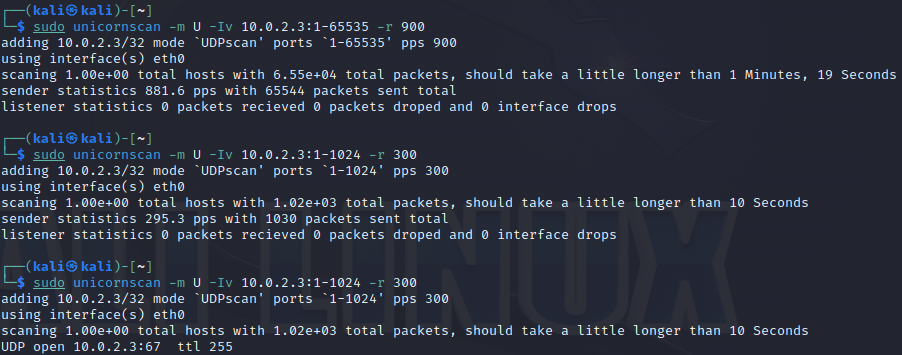
\includegraphics[width=0.7\textwidth]{capitoli/figure/unicornscan-multiple.png}
    \caption{Risultato scansioni \emph{UDP} aggiuntive con \texttt{unicornscan}}
    \label{fig:unicornscan-multiple}
\end{figure}

Da questi risultati emerge che con ulteriori scansioni, questa volta effettuate sull'host \emph{10.0.2.3}, tale porta viene rilevata solo una volta.

Tuttavia, tornado per un attimo al risultato ottenuto nella Figura \ref{fig:unicornscan-scan}, alla porta 67 del protocollo \emph{UDP} viene associato un servizio denominato \textbf{bootps} (come si evince anche dall'elenco delle porte note \cite{rfc1340}). Effettuando delle ricerche a proposito, quello che si scopre è che il servizio in realtà si chiama \textbf{BOOTSTRAP} ed è l'equivalente \emph{UDP} del servizio \textbf{DHCP} \cite{bootp}. A tal proposito, immaginando che il comportamento sia molto simile a \textbf{DHCP}, è lecito supporre che l'host \emph{10.0.2.3} periodicamente invii dei pacchetti \emph{UDP} a tutti gli host della rete (ricordando che esso è un host "\emph{fittizio}" della rete virtuale). A questo punto, essendo che per stabilire se una porta \emph{UDP} è aperta ci si aspetta un pacchetto \emph{UDP} in risposta oppure nessuna risposta (se si riceve un messaggio \emph{ICMP} allora la porta è chiusa), nel momento in cui riceviamo una risposta \emph{UDP} allora etichettiamo la porta di origine come aperta \cite{udp-scan}. Quindi \texttt{unicornscan}, per come è stato realizzato, non scarta i messaggi \emph{UDP} provenienti da altri host (fortunatamente indica l'host di origine nel risultato) e, per tale ragione, se un altro host invia un pacchetto \emph{UDP} alla macchina \textbf{Kali} allora \texttt{unicornscan} non perde occasione di segnalare porta e host di orgine del pacchetto etichettandola come \emph{aperta} anche se il pacchetto non proviene dall'host interessato dalla scansione \cite{unicornscan-doc}.

\subsubsection{Osservazioni finali}
In virtù delle osservazioni fatte e dai risultati ottenuti dalla scansione, possiamo quindi stabilire che l'asset non ha porte \emph{UDP} aperte e che l'host \emph{10.0.2.3} ha la porta \emph{67} aperta con la quale invia pacchetti \textbf{bootps} a tutti gli host della rete per indicare tramite \emph{UDP} qual è il loro rispettivo indirizzo IP.

\section{Vulnerability Mapping}
Ora che sono stati rilevati i vari servizi attivi sull'asset si può procedere con l'analisi delle vulnerabilità presenti.
\subsection{Scansione vulnerabilità con \emph{Nessus}}
La prima scansione delle vulnerabilità presenti è stata realizzata con \emph{Nessus}, strumento commerciale di analisi delle vulnerabilità molto potente che, fortunatamente, offre un piano gratuito (seppur abbastanza limitato). Una volta avviato lo strumento e aggiornato, è stata scelta l'opzione \textbf{basic scan} ed è stato creato un task di analisi con scansione su \textbf{tutte le porte} sul solo asset.

In seguito all'esecuzione del task, un primo risultato grafico dei rilevamenti è il seguente:

\begin{figure}[h]
    \centering
    \begin{subfigure}{0.9\textwidth}
        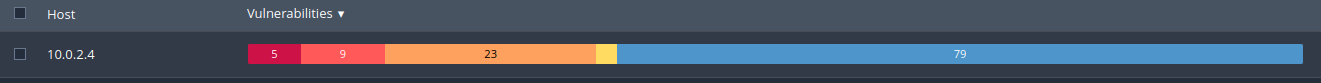
\includegraphics[width=1\textwidth]{capitoli/figure/nessus-scan-1.png}
        \caption{Rilevamenti di \emph{Nessus}}
        \label{fig:nessus-scan-1}
    \end{subfigure}
    \begin{subfigure}{0.4\textwidth}
        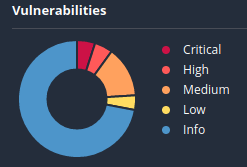
\includegraphics[width=1\textwidth]{capitoli/figure/nessus-scan-2.png}
        \caption{Grafico a torta dei rilevamenti di \emph{Nessus}}
        \label{fig:nessus-scan-2}
    \end{subfigure}
    \caption{Risultati di \emph{Nessus}}
\end{figure}

I risultati dettagliati della scansione sono consultabili nella cartella \emph{Report} aprendo il file con nome \textbf{De-ICE\_scan\_nessus.pdf} mentre il solo elenco è presente nel file \textbf{De-ICE\_scan\_nessus-elenco.pdf}.\\

\subsection{\emph{Wrap-up} dei due report}
Quello che possiamo notare dalla consultazione dei due report è che i due tool hanno rilevato problematiche differenti. Ad esempio, \emph{Nessus} ha identificato una grave problematica di \textbf{ProFTPD} che permette l'accesso non autorizzato al file system e la presenza di una versione di \emph{SSL} affetta dalla problematica conosciuta come \textbf{HeartBleed}, mentre \emph{OpenVAS} ha rilevato che il Sistema Operativo è deprecato e ha raggiunto l'\textbf{End of Life} e che la versione di \emph{SSL/TLS} utilizzata sfrutta cifrari che sono crittograficamente deboli al giorno d'oggi.

\subsection{Scansione vulnerabilità con \emph{OpenVAS}}
In seguito alla scansione con \emph{Nessus}, è stata realizzata una scansione anche con \emph{OpenVAS}, altro strumento molto potente e liberamente utilizzabile. Anche in questo caso è stato realizzato un task di scansione che prevedesse la scansione di tutte le porte presenti sull'asset, personalizzando opportunamente i vari campi. In seguito all'esecuzione della scansione, durata molto più tempo rispetto alla scansione di \emph{Nessus}, una vista grafica dei risultati è illustrato nella Figura \ref{fig:openvas}:

\begin{figure}[h]
    \centering
    \begin{subfigure}{0.8\textwidth}
        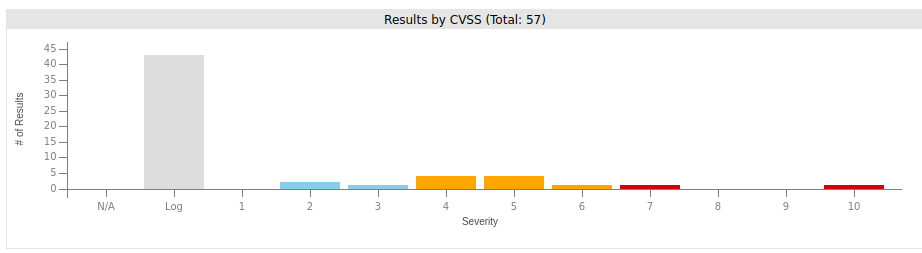
\includegraphics[width=1\textwidth]{capitoli/figure/openvas-1.png}
        \caption{Istogramma rilevamenti di \emph{OpenVAS} per gravità}
        \label{fig:openvas-1}
    \end{subfigure}
    \begin{subfigure}{0.7\textwidth}
        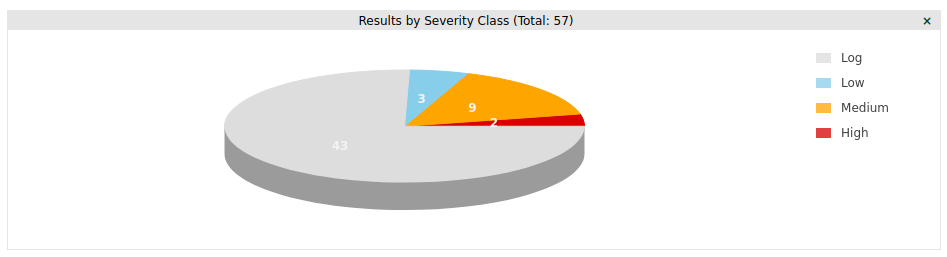
\includegraphics[width=1\textwidth]{capitoli/figure/openvas-2.png}
        \caption{Grafico a torta dei rilevamenti di \emph{OpenVAS}}
        \label{fig:openvas-2}
    \end{subfigure}
    \caption{Risultati di \emph{OpenVAS}}
    \label{fig:openvas}
\end{figure}

A differenza di \emph{Nessus}, in questo caso è stata impostata anche una soglia di \textbf{Quality of Detection}, la quale permette di escludere dal resoconto possibili falsi positivi rilevati per mezzo del motore euristico di \emph{OpenVAS}. Si è deciso, a questo scopo, di lasciare la minima \emph{QoD} di default che è $70\%$, la quale ha permesso di escludere circa 200 rilevamenti che, molto probabilmente, sono dei semplici falsi positivi. Anche in questo caso i risultati dettagliati sono consultabili nella cartella \emph{Report} aprendo il file \textbf{De-ICE\_scan\_openvas.pdf}

\subsection{Scansione vulnerabilità web con \emph{Nessus}}
Essendo che l'asset offre anche il servizio \textbf{web}, si è vista la necessità di effettuare delle scansioni \emph{ad-hoc} per questo tipo di servizio essendo che sono molto diffuse le vulnerabilità di questo tipo e, allo stesso tempo, possono essere anche molto pericolose.\\
Dal momento che \emph{Nessus} offre una tipologia apposita di task per le scansioni web, ne è stato realizzato uno che effettuasse un'analisi quanto più esaustiva possibile modificando opportunamente i parametri di scansione.

In seguito all'esecuzione del task, una prima vista grafica dei risultati è rappresentata di seguito nella Figura \ref{fig:nessus-web}.

\begin{figure}[h]
    \centering
    \begin{subfigure}{0.9\textwidth}
        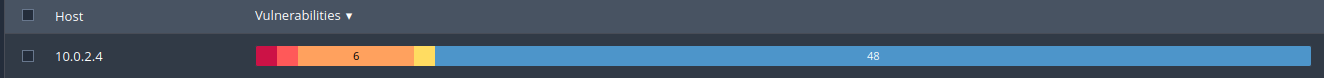
\includegraphics[width=1\textwidth]{capitoli/figure/nessus-web-1.png}
        \caption{Rilevamenti web di \emph{Nessus}}
        \label{fig:nessus-web-1}
    \end{subfigure}
    \begin{subfigure}{0.4\textwidth}
        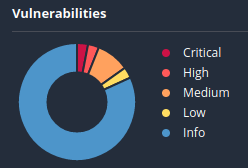
\includegraphics[width=1\textwidth]{capitoli/figure/nessus-web-2.png}
        \caption{Grafico a torta dei rilevamenti web di \emph{Nessus}}
        \label{fig:nessus-web-2}
    \end{subfigure}
    \caption{Risultati web di \emph{Nessus}}
    \label{fig:nessus-web}
\end{figure}

Anche in questo caso un report dettagliato dove consultare le vulnerabilità rilevate è presente nella cartella \emph{Report} con il nome \textbf{De-ICE\_nessus\_web.pdf}, così come anche un elenco dei rilevamenti con il nome \textbf{De-ICE\_nessus\_web-elenco.pdf}.

\subsection{Altre scansioni di vulnerabilità web}
In seguito alla scansione effettuata con \emph{Nessus}, si è deciso di effettuare ulteriori scansioni sfruttando altri tool, alcuni anche specifici per determinati contenuti.

\subsubsection{Scansione con \texttt{whatweb}}
Per verificare l'eventuale presenza di \textbf{CMS} come \emph{Wordpress} o \emph{Joomla}, i quali richiedono ulteriori approfondimenti con strumenti specifici, si è deciso di utilizzare lo strumento \texttt{whatweb}, incaricato di rilevare la presenza di questi dietro un servizio web.

Per eseguire lo strumento basta lanciare il seguente comando:
\begin{lstlisting}[language=bash]
    whatweb 10.0.2.4
\end{lstlisting}

Eseguendo il comando, il risultato che si ottiene è il seguente:
\begin{figure}[h]
    \centering
    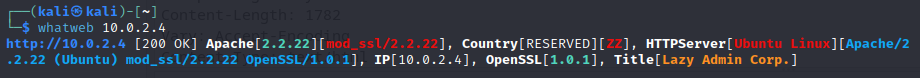
\includegraphics[width=0.9\textwidth]{capitoli/figure/whatweb.png}
    \caption{Risultato esecuzione di \texttt{whatweb}}
    \label{fig:whatweb}
\end{figure}

Dal momento che non sono stati rilevati \textbf{CMS}, non si approfondirà ulteriormente l'argomento.

\subsubsection{Scansione con \texttt{wafw00f}}
In vista dell'esecuzione di scansioni di vulnerabilità web, potrebbe essere conveniente accertarsi della presenza o meno di un \textbf{Web Application Firewall}. In realtà, essendo che l'asset è una macchina virtuale posta all'interno di una rete virtuale, difficilmente potrebbe essere configurata per operare, ad esempio, con un \emph{WAF} come \emph{Cloudflare} o simili. Tuttavia, essendo che nelle prime scansioni si è notato che le porte non rilevate come aperte erano tutte filtrate, vale la pena di approfondire sulla presenza di un eventuale \emph{WAF}.
Per rilevare la presenza di un \textbf{Web Application Firewall}, si è deciso di utilizzare \texttt{wafw00f}. Per eseguire lo strumento basta lanciare il seguente comando:
\begin{lstlisting}[language=bash]
    wafw00f 10.0.2.4
\end{lstlisting}

In seguito all'esecuzione del comando, il risultato è il seguente:
\begin{figure}[h]
    \centering
    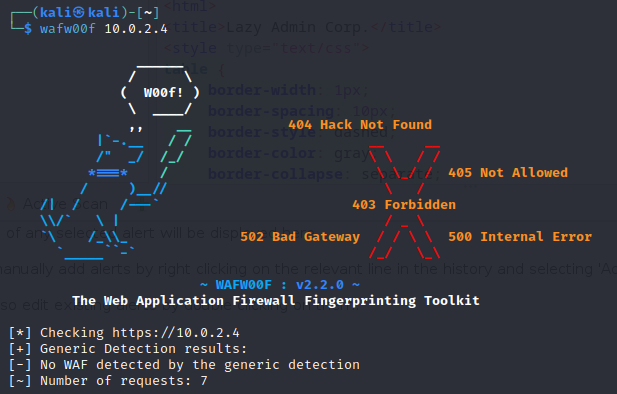
\includegraphics[width=0.9\textwidth]{capitoli/figure/wafw00f.png}
    \caption{Risultato esecuzione di \texttt{wafw00f}}
    \label{fig:wafw00f}
\end{figure}

Dal risultato ottenuto, possiamo concludere che non sono presenti \emph{WAF} (come ipotizzato in precedenza) e quindi non sarà necessario prendere particolari precauzioni nelle fasi successive.

\subsubsection{Scansione con \emph{OWASP ZAP}}

\subsubsection{Scansione con \texttt{nikto}}

\subsection{Rilevamento path visitabili con \texttt{dirb}}

\subsection{Ulteriore scansione con \texttt{paros}}